\documentclass{beamer}
\usetheme[
  block=fill,
  background=dark,
  titleformat=smallcaps,
  progressbar=frametitle,
  numbering=none,
]{metropolis}

%----------------------------------------------------------------------------
% From dyck-paper
%----------------------------------------------------------------------------
\usepackage{mwe,tikz}\usepackage[percent]{overpic}
\usepackage{caption}
\usepackage{epigraph}
% Math
\usepackage{amsmath}
\usepackage{amssymb}
\usepackage{stmaryrd}
% Code listing
\usepackage{minted}
%\usemintedstyle{friendly}
\usemintedstyle{tango}
\usepackage{algorithm}
\usepackage[noend]{algpseudocode}
% Colors
\usepackage{xcolor}
\colorlet{CodeBg}{gray!90}
\usepackage{color, colortbl}
\definecolor{Gray}{rgb}{0.9,0.9,0.9}
\definecolor{bblue}{HTML}{1D577A}
\definecolor{rred}{HTML}{C03425}
\definecolor{ggreen}{HTML}{8BB523}
\definecolor{ppurple}{HTML}{6B1B7F}
\definecolor{pblack}{HTML}{000000}
\definecolor{pyellow}{HTML}{C0B225}
% Graphs
\usepackage{tikz}
\usetikzlibrary{calc}
\usetikzlibrary{trees}
\usetikzlibrary{positioning}
\usepackage{pgfplots}
% Graphics
\usepackage{graphics}
\graphicspath{{figures/}} % Location of the graphics files

\newcommand\todo[1]{\textcolor{red}{#1}}
\newcommand{\w}[1]{\textit{"#1"}}
\newcommand{\sm}[1]{\text{\small{#1}}}
\newcommand\s{\textsc}

\newcommand{\Order}[5]{
	\[
	\mathcal{#1}_{#5}\llbracket #2 \leftarrow #3 \mid \{ #4 \} \rrbracket.
	\]
}
\newcommand{\Orderr}[5]{
	\mathcal{#1}_{#5}\llbracket #2 \leftarrow #3 \mid \{ #4 \} \rrbracket.
}
\newcommand{\Ord}[4]{\Order{O}{#1}{#2}{#3}{#4}}
\newcommand{\Or}[4]{\Orderr{O}{#1}{#2}{#3}{#4}}
\newcommand{\Con}[4]{\Order{C}{#1}{#2}{#3}{#4}}

% Box macro
\newcommand{\ex}[2]{
  \vfill
  \begin{alertblock}{#1}
    #2
  \end{alertblock}
}
\newcommand\tsc[1]{\alert{\textsc{#1}}}
\newcommand\charth{4cm}
\newcommand\bb[1]{\scriptsize \textcolor{black}{$n=#1$}}
\newcommand\rr[1]{\textcolor{rred}{#1}}
\newcommand\gr[1]{\textcolor{ggreen}{#1}}
%----------------------------------------------------------------------------

% Beamer
\title{$D^3$ as a 2-MCFL}
\subtitle{}
\author{Orestis Melkonian, Konstantinos Kogkalidis}
\date{January 25, 2018}
\institute{Universiteit Utrecht}

\begin{document}
	\maketitle

	\begin{frame}{}
	\begin{center}
	\vspace{1cm}
	\colorbox{white}{
    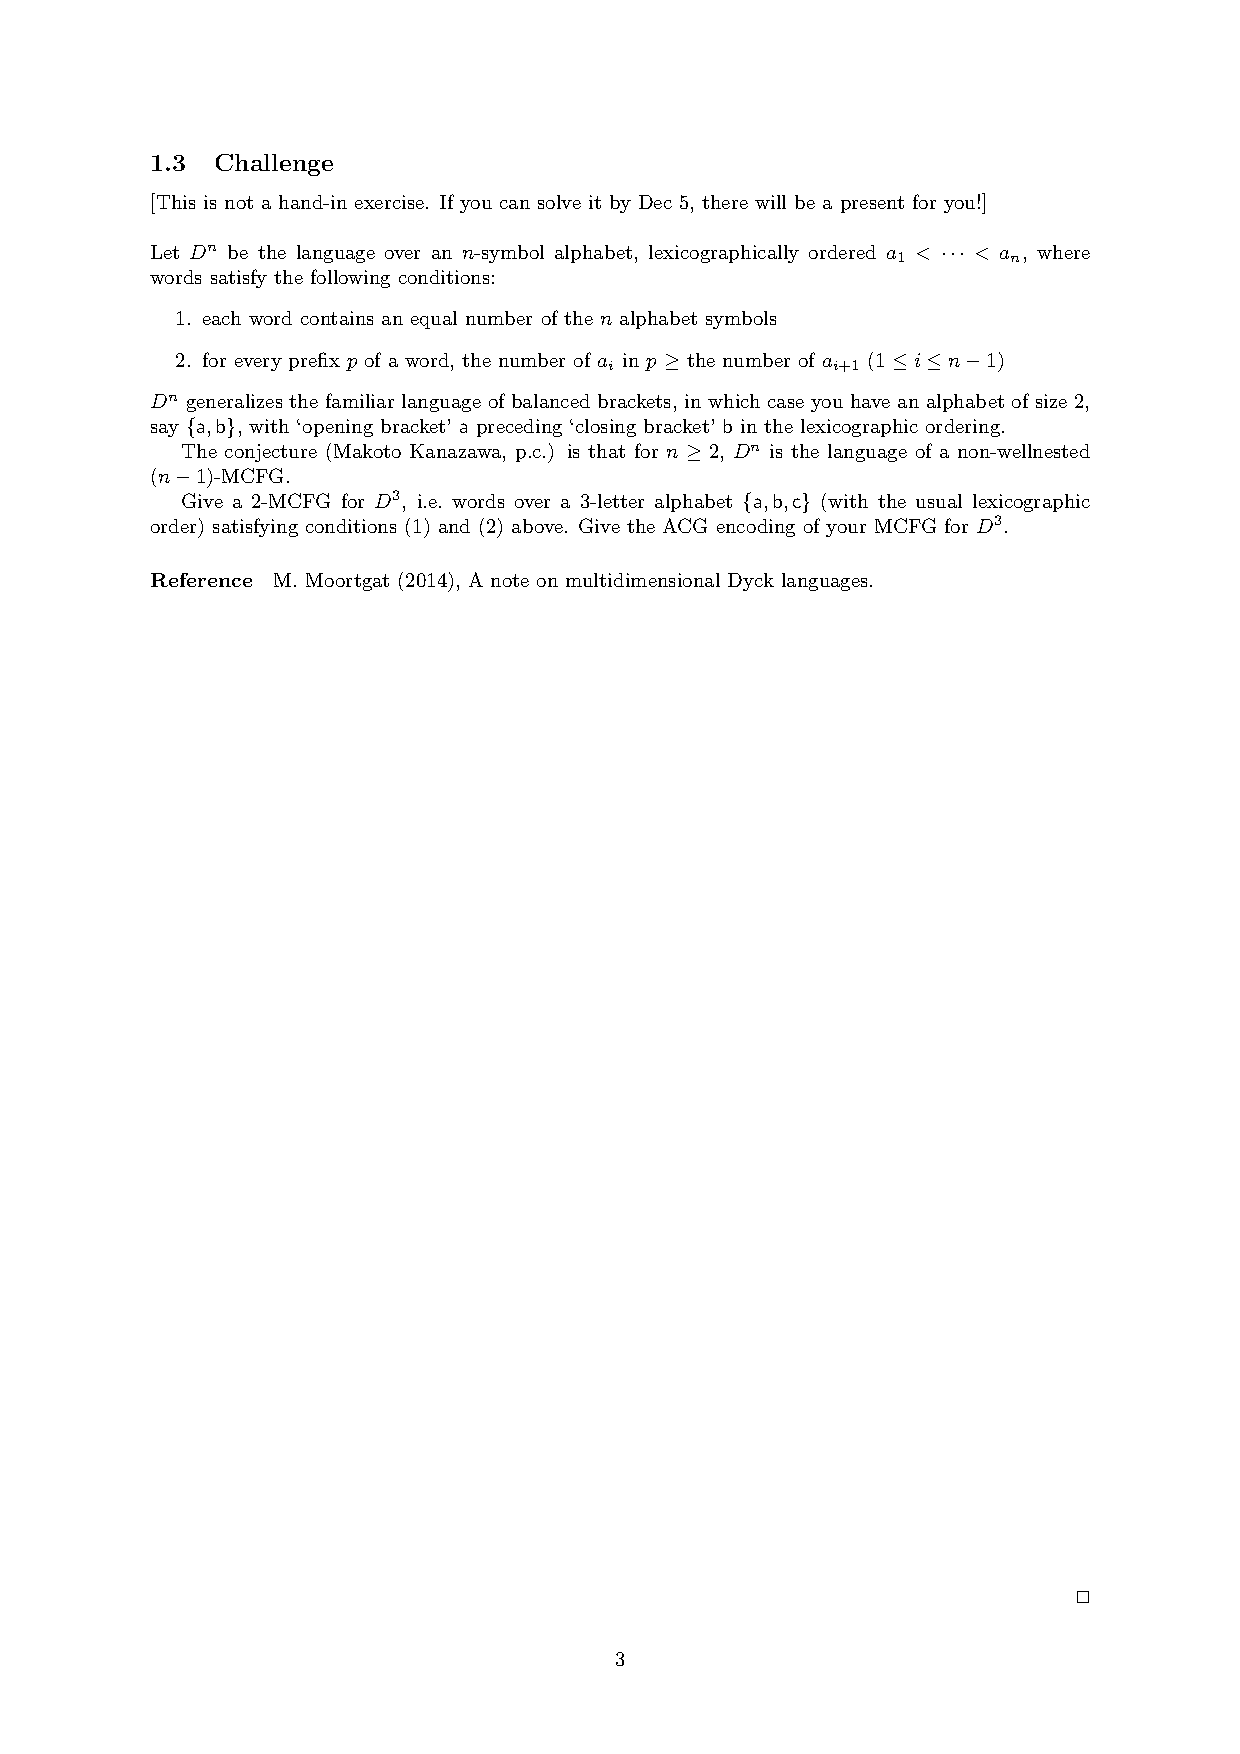
\includegraphics[clip, trim=1cm 18cm 1cm 1cm, scale=.55]{quiz.pdf}}
	\end{center}
	\end{frame}

	\begin{frame}{Some examples}
		\hspace{1cm}
		\begin{minipage}{.4\textwidth}
		\textsc{Dyck words}
		\begin{itemize}
			\item \textcolor{ggreen}{abc}
			\item \textcolor{ggreen}{aabbcc}
			\item \textcolor{ggreen}{abcabcabacbc}
		\end{itemize}
		\end{minipage}
		\pause
		\begin{minipage}{.4\textwidth}
		\textsc{Non-dyck words}
		\begin{itemize}
			\item \textcolor{rred}{aabb}
			\pause
			\item \textcolor{rred}{aabbbcc}
			\pause
			\item \textcolor{rred}{abcacb}
		\end{itemize}
		\end{minipage}
		\vspace{1cm}
		\pause
		\begin{figure}[h!]
		\centering
		
\begin{tikzpicture}[every node/.style={anchor=base},xscale=.25,yscale=.4]
			\node (n0) at (0,0) {$a$};
			\node (n1) at (1,0) {$b$};
			\node (n2) at (2,0) {$a$};
			\node (n3) at (3,0) {$b$};
			\node (n4) at (4,0) {$a$};
			\node (n5) at (5,0) {$c$};
			\node (n6) at (6,0) {$b$};
			\node (n7) at (7,0) {$c$};
			\node (n8) at (8,0) {$a$};
			\node (n9) at (9,0) {$b$};
			\node (n10) at (10,0) {$c$};
			\node (n11) at (11,0) {$c$};
			\pause
			\draw (n0) edge [thick, rred, bend left=90] (n1);
			\draw (n1) edge [thick, rred, bend right=90] (n5);
			\pause
			\draw (n2) edge [thick, ggreen, bend left=90] (n3);
			\draw (n3) edge [thick, ggreen, bend right=90] (n7);
			\pause
			\draw (n4) edge [thick, bblue, bend left=90] (n6);
			\draw (n6) edge [thick, bblue, bend right=90] (n10);
			\pause
			\draw (n8) edge [thick, pyellow, bend left=90] (n9);
			\draw (n9) edge [thick, pyellow, bend right=90] (n11);
		\end{tikzpicture}
		\caption*{First-match policy}
		\end{figure}
	\end{frame}

	\begin{frame}{G$_0$: Grammar of triple insertions}
		\begin{figure}[h!]
		\begin{align}
		\setcounter{equation}{0}
		\s{S}(xy) \leftarrow \s{W}(x,y)&. \\
		\s{W}(\epsilon, xy\textbf{abc}) \leftarrow \s{W}(x,y)&. \\
		\s{W}(\epsilon, x\textbf{a}y\textbf{bc}) \leftarrow \s{W}(x,y)&. \\
		...... \nonumber \\
		\setcounter{equation}{59}
		\s{W}(\textbf{ab}x\textbf{c}y, \epsilon) \leftarrow \s{W}(x,y)&. \\
		\s{W}(\textbf{abc}xy, \epsilon) \leftarrow \s{W}(x,y)&. \\
		\s{W}(\epsilon, \textbf{abc})&. \\
		\s{W}(\textbf{a}, \textbf{bc})&. \\
		\s{W}(\textbf{ab}, \textbf{c})&. \\
		\s{W}(\textbf{abc}, \epsilon)&.
		\end{align}
		\end{figure}
	\end{frame}

	\begin{frame}{G$_0$: Grammar of triple insertions}
		\begin{figure}[h!]
		\centering
		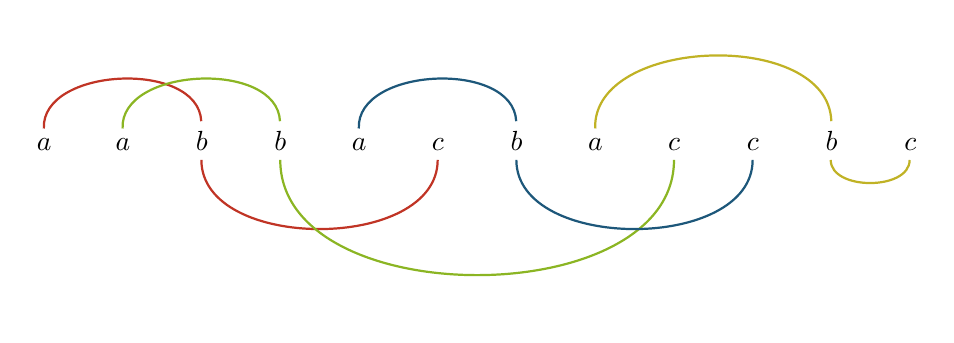
\begin{tikzpicture}[every node/.style={anchor=base}]
			\node (n0) at (0,0) {$a$};
			\node (n1) at (1,0) {$a$};
			\node (n2) at (2,0) {$b$};
			\node (n3) at (3,0) {$b$};
			\node (n4) at (4,0) {$a$};
			\node (n5) at (5,0) {$c$};
			\node (n6) at (6,0) {$b$};
			\node (n7) at (7,0) {$a$};
			\node (n8) at (8,0) {$c$};
			\node (n9) at (9,0) {$c$};
			\node (n10) at (10,0) {$b$};
			\node (n11) at (11,0) {$c$};
			\pause
			\draw (n0) edge [thick, rred, bend left=90] (n2);
			\draw (n2) edge [thick, rred, bend right=90] (n5);
			\pause
			\draw (n1) edge [thick, ggreen, bend left=90] (n3);
			\draw (n3) edge [thick, ggreen, bend right=90] (n8);
			\pause
			\draw (n4) edge [thick, bblue, bend left=90] (n6);
			\draw (n6) edge [thick, bblue, bend right=90] (n9);
			\pause
			\draw (n7) edge [thick, pyellow, bend left=90] (n10);
			\draw (n10) edge [thick, pyellow, bend right=90] (n11);
		\end{tikzpicture}
		\caption*{Straddling counter-example}
		\end{figure}
	\end{frame}

  	\begin{frame}{Meta-grammars: Introduction}
	  	\vspace{.7cm}
	  	\center \tsc{Notation}
  		\[
  			\Or{conclusion}{premises}{partial\ orderings\ of\ inserted\ elements}{m}
  		\]
  		\vspace{.1cm}
  		\pause
  		\begin{center}\tsc{Meta-grammar G$_1$}\end{center}
  		  \[ \left . \
  		  	\begin{array}{ll}
				\Or{W}{\epsilon}{a < b < c}{2} \\
               		\Or{W}{W_{xy}}{x < y,\ a < b < c}{2}
	           \end{array}
           	\right\} \
           	\begin{array}{c}
           		\textsc{triple} \\
	           	\textsc{insertion}
     		      \end{array}
		  \]
  		\pause
  		\hspace{-4cm} \textcolor{ggreen}{+} \vspace{-3mm}
  		\[ \left . \
  		   \hspace{.75cm}
  		   \begin{array}{ll}
		       \Or{W}{W_{xy}, W_{zw}}{x < y,\ z < w}{2}
         	   \end{array}
             \right\} \
             \begin{array}{c}
         		  \textsc{interleaving} \\
           	  \textsc{words}
	        \end{array}
		\]
  		\vspace{.7cm}
  	\end{frame}

  	\begin{frame}{G$_2$: Adding states}
   	\small
   	\begin{flalign*}
 		&\left . \ \begin{array}{lr}
					\Or{A^+}{\epsilon}{a}{2} \\
					\Or{B^+}{\epsilon}{b}{2} \\
					\Or{C^+}{\epsilon}{c}{2}
           \end{array}
           \right\} \tsc{base cases} \\
  		&\noindent\rule{11cm}{0.4pt}\\
 		&\left . \ \begin{array}{lr}
					\Or{C^-}{A^+, B^+}{x < y < z < w}{2} \\
					\Or{B^-}{A^+, C^+}{x < y < z < w}{2} \\
					\Or{A^-}{B^+, C^+}{x < y < z < w}{2} \\
					\Or{A^+}{C^-, B^-}{x < y < z < w}{2} \\
					\Or{B^+}{C^-, A^-}{x < y < z < w}{2} \\
					\Or{C^+}{B^-, A^-}{x < y < z < w}{2} \\
					\forall \ \s{K} \in \mathcal{S} \setminus \s{W}:\ \Or{\s{K}}{\s{K}_{xy}, \s{W}_{zw}}{x < y,\ z < w}{2}
           \end{array}
           \right\} \tsc{combinations} \\
		&\noindent\rule{11cm}{0.4pt}\\
  		&\left . \ \begin{array}{lr}
					\Or{W}{A^+, A^-}{x < y < z < w}{2} \\
					\Or{W}{C^-, C^+}{x < y < z < w}{2}
           \end{array}
           \right\} \tsc{closures}
	\end{flalign*}
  	\end{frame}

  	\begin{frame}{G$_3$: G$_2$ + Universal triple insertion}
  	\begin{align*}
  		&\text{G}_3 = \text{G}_2\ \textcolor{ggreen}{+}\ \forall \ \s{K} \in \mathcal{S} \setminus \s{W}:\\
&\hspace{3cm}\Or{\s{K}}{\s{K}_{xy}}{x < y,\ a < b < c}{2}
  	\end{align*}
  	\end{frame}

{\usebackgroundtemplate{%
  
\includegraphics[width=\paperwidth,height=\paperheight]{demo.png}}
	\begin{frame}{Demo}
%	   \centering
%	   \begin{overpic}[scale=0.3]{demo.png}
%	     \put(20,10){
\includegraphics[scale=0.2]{demo.png}}
%	     \put(35,20){
\includegraphics[scale=0.1]{demo.png}}
%	   \end{overpic}
  	\end{frame}
}
  	\begin{frame}{Refining states}
  		\center \tsc{Example}
  		\begin{figure}[h!]
		\centering
		\begin{tikzpicture}[every node/.style={anchor=base}, scale=.9]
			\node (c) at (0,0) {$A^{+}(x, y)$};
			\node (l) at (-1,-1) {$A^{+}_{left}$};
			\node (r) at (1,-1) {$A^{+}_{right}$};
			\draw (c) edge [->, mLightBrown, thick] (l);
			\draw (c) edge [->, mLightBrown, thick] (r);
			\pause
			\node (v) at (0,-1.6) {$\vdots$};
			\node (cc) at (0,-2.3) {$C^{-}(x, y)$};
			\node (ll) at (-2,-3.3) {$C^{-}_{left}$};
			\node (rr) at (2,-3.3) {$C^{-}_{right}$};
			\node (lr) at (0,-3.8) {$C^{-}_{left,\ right}$};
			\draw (cc) edge [->, mLightBrown, thick] (ll);
			\draw (cc) edge [->, mLightBrown, thick] (rr);
			\draw (cc) edge [->, mLightBrown, thick] (lr);
		\end{tikzpicture}
		\end{figure}
		\vspace{2.2cm}
  	\end{frame}
  	\begin{frame}{Refining states}
  		\center \tsc{Example}
  		\begin{figure}[h!]
		\centering
		\begin{tikzpicture}[every node/.style={anchor=base}, scale=.9]
			\node (c) at (0,0) {$A^{+}(x, y)$};
			\node (l) at (-1,-1) {$A^{+}_{left}$};
			\node (r) at (1,-1) {$A^{+}_{right}$};
			\draw (c) edge [->, mLightBrown, thick] (l);
			\draw (c) edge [->, mLightBrown, thick] (r);
			\node (v) at (0,-1.6) {$\vdots$};
			\node (cc) at (0,-2.3) {$C^{-}(x, y)$};
			\node (ll) at (-2,-3.3) {$C^{-}_{left}$};
			\node (rr) at (2,-3.3) {$C^{-}_{right}$};
			\node (lr) at (0,-3.8) {$C^{-}_{left,\ right}$};
			\draw (cc) edge [->, mLightBrown, thick] (ll);
			\draw (cc) edge [->, mLightBrown, thick] (rr);
			\draw (cc) edge [->, mLightBrown, thick] (lr);
		\end{tikzpicture}
		\end{figure}
		\center \tsc{Why? \pause \\New orders in interactions}
		\[ C^-(xz,\ wy) \leftarrow A^{+}_{left}(x,\ y),\ B^+(z,\ w).
		\]
  	\end{frame}

  	\begin{frame}{Refining states: Interactions}
  		\centering
		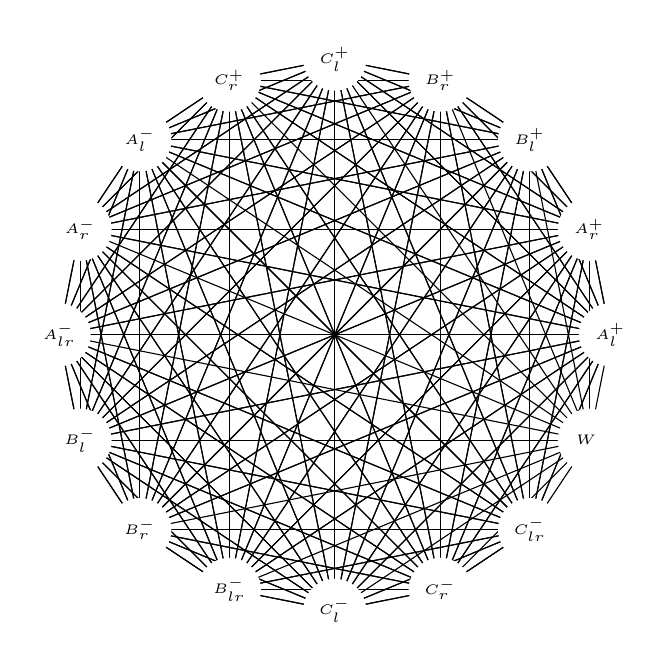
\begin{tikzpicture}[scale=.7]
		  \foreach \x /\alph/\name in {
		  		0/n1/$A^{+}_{l}$,
		  		22.5/n2/$A^{+}_{r}$,
		  		45/n3/$B^{+}_{l}$,
		  		67.5/n4/$B^{+}_{r}$,
		  		90/n5/$C^{+}_{l}$,
		  		112.5/n6/$C^{+}_{r}$,
		  		135/n7/$A^{-}_{l}$,
		  		157.5/n8/$A^{-}_{r}$,
		  		180/n9/$A^{-}_{lr}$,
		  		202.5/n10/$B^{-}_{l}$,
		  		225/n11/$B^{-}_{r}$,
		  		247.5/n12/$B^{-}_{lr}$,
		  		270/n13/$C^{-}_{l}$,
		  		292.5/n14/$C^{-}_{r}$,
		  		315/n15/$C^{-}_{lr}$,
		  		337.5/n16/$W$
		  }{
		  	\node[] (\alph) at (\x:5cm) {};
		  }
		  \foreach \alpha in {n1,n2,n3,n4,n5,n6,n7,n8,n9,n10,n11,n12,n13,n14,n15,n16}%
		  {%
		  \foreach \alphb in {n1,n2,n3,n4,n5,n6,n7,n8,n9,n10,n11,n12,n13,n14,n15}%
		  {%
		   \draw (\alpha) edge (\alphb);%
		  }}
		  \foreach \x /\alph/\name in {
		  		0/n1/$A^{+}_{l}$,
		  		22.5/n2/$A^{+}_{r}$,
		  		45/n3/$B^{+}_{l}$,
		  		67.5/n4/$B^{+}_{r}$,
		  		90/n5/$C^{+}_{l}$,
		  		112.5/n6/$C^{+}_{r}$,
		  		135/n7/$A^{-}_{l}$,
		  		157.5/n8/$A^{-}_{r}$,
		  		180/n9/$A^{-}_{lr}$,
		  		202.5/n10/$B^{-}_{l}$,
		  		225/n11/$B^{-}_{r}$,
		  		247.5/n12/$B^{-}_{lr}$,
		  		270/n13/$C^{-}_{l}$,
		  		292.5/n14/$C^{-}_{r}$,
		  		315/n15/$C^{-}_{lr}$,
		  		337.5/n16/$W$
		  }{
		  	\node[circle,inner sep=0pt,minimum size=8mm,fill=white] (\alph) at (\x:5cm) {\tiny \textcolor{black}{\name}};
		  }
		 \end{tikzpicture}
  	\end{frame}

  	\begin{frame}{G$_4$: Automatic Rule Inference}
  		\center \tsc{State descriptors $\mathcal{D}$}\\
	  	\begin{minipage}{.49\textwidth}
		\begin{align*}
		\s{W} &\mapsto (\epsilon, \epsilon) \\
		\s{A}^+_{l} &\mapsto (a, \epsilon) \\
		\s{A}^+_{r} &\mapsto (\epsilon, a) \\
		\s{B}^+_{l} &\mapsto (b, \epsilon) \\
		\s{B}^+_{r} &\mapsto (\epsilon, b) \\
		\s{C}^+_{l} &\mapsto (c, \epsilon) \\
		\s{C}^+_{r} &\mapsto (\epsilon, c) \\
		\s{A}^-_{l} &\mapsto (bc, \epsilon)
		\end{align*}
		\end{minipage}
		\begin{minipage}{.49\textwidth}
		\begin{align*}
		\s{A}^-_{r} &\mapsto (\epsilon, bc) \\
		\s{A}^-_{lr} &\mapsto (b, c) \\
		\s{B}^-_{l} &\mapsto (ac, \epsilon) \\
		\s{B}^-_{r} &\mapsto (\epsilon, ac) \\
		\s{B}^-_{lr} &\mapsto (a, c) \\
		\s{C}^-_{l} &\mapsto (ab, \epsilon) \\
		\s{C}^-_{r} &\mapsto (\epsilon, ab) \\
		\s{C}^-_{lr} &\mapsto (a, b)
		\end{align*}
		\end{minipage}
  	\end{frame}

  	\begin{frame}{Automatic Rule Inference: Example}
  		\center \tsc{Case of} $\s{A}^-_{lr}(x_{\textcolor{ggreen}{b}},\ y_{\textcolor{ggreen}{c}})$ \tsc{+} $\s{B}^-_{lr}(z_{\textcolor{ggreen}{a}},\ w_{\textcolor{ggreen}{c}})$
		\begin{figure}[h!]
		\centering
		\begin{tikzpicture}[every node/.style={anchor=base}, scale=.9]
			\node (i0) at (-1,1) {\textsc{\underline{permutation}}};
			\node at (-1,0) {$\vdots$};
			\node (p1) at (-1,-1) {$(zxw,\ y)$};
			\node at (-1,-2) {$\vdots$};
			\node (p2) at (-1,-3) {$(xzw,\ y)$};
			\node at (-1,-4) {$\vdots$};
			\pause
			\node (i1) at (3,1) {\textsc{\underline{descriptor}}};
			\node at (3,0) {$\vdots$};
			\node (d1) at (3,-1) {$(abc,\ c)$};
			\node at (3,-2) {$\vdots$};
			\node (d2) at (3,-3) {$(bac,\ c)$};
			\node at (3,-4) {$\vdots$};
			\draw (p1) edge [->, mLightBrown, thick] (d1);
			\draw (p2) edge [->, mLightBrown, thick] (d2);
			\pause
			\node (i2) at (7,1) {\textsc{\underline{eliminated}}};
			\node at (7,.25) {$\vdots$};
			\node (e1) at (7,-.5) {$(c,\ \epsilon) \mapsfrom \s{C}^+_{l}$};
			\node (e2) at (7,-1.5) {$(\epsilon,\ c) \mapsfrom \s{C}^+_{r}$};
			\node at (7,-2.25) {$\vdots$};
			\node (e3) at (7,-3) {$(bac,\ c) \ \notin\ \mathcal{D} $};
			\node at (7,-3.75) {$\vdots$};
			\draw (d1) edge [->, mLightBrown, thick] (e1);
			\draw (d1) edge [->, mLightBrown, thick] (e2);			
			\draw (d2) edge [->, mLightBrown, thick] (e3);
		\end{tikzpicture}
		\end{figure}
  	\end{frame}

	\metroset{background=light}
  	\begin{frame}{Results}
  	\begin{figure}[h!]
  		% Counter-examples
		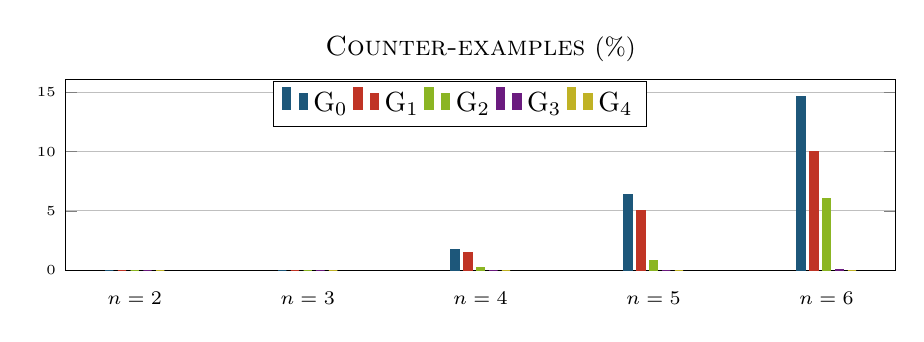
\begin{tikzpicture}
		    \begin{axis}[
		    		black,
		        width  = \textwidth,
		        height = \charth,
		        major x tick style = transparent,
		        ybar=4*\pgflinewidth,
		        bar width=3pt,
		        ymajorgrids = true,
		        ylabel = {\textsc{Counter-examples} \small (\%)},
		        every tick label/.append style={font=\tiny},
		        every axis x label/.style={
		        		  black,
		  			  at={(ticklabel* cs:1.05)},
		  			  anchor=west,
		  			  },
			   	  every axis y label/.style={black,at={(current axis.north)},above=1mm},
		        symbolic x coords={\bb{2},\bb{3},\bb{4},\bb{5},\bb{6}},
		        xtick = data,
		        scaled y ticks = false,
		        enlarge x limits=0.1,
		        ymin=0,
		        legend cell align=left,
		        legend style={
		        		at={(.25,.75)},
						anchor=south west,
						legend columns=-1
					},
		    ]
		        \addplot[style={bblue,fill=bblue,mark=none}]
		            coordinates {(\bb{2}, 0.0) (\bb{3},0.0) (\bb{4},1.7) (\bb{5},6.4) (\bb{6},14.6)};
		        \addplot[style={rred,fill=rred,mark=none}]
		            coordinates {(\bb{2},0) (\bb{3},0) (\bb{4},1.5) (\bb{5},5) (\bb{6},10)};
		        \addplot[style={ggreen,fill=ggreen,mark=none}]
		            coordinates {(\bb{2},0) (\bb{3},0) (\bb{4},0.2) (\bb{5},0.8) (\bb{6},6)};
		        \addplot[style={ppurple,fill=ppurple,mark=none}]
		            coordinates {(\bb{2},0) (\bb{3},0) (\bb{4},0) (\bb{5},0) (\bb{6},0.02)};
		        \addplot[style={pyellow,fill=pyellow,mark=none}]
		            coordinates {(\bb{2},0) (\bb{3},0) (\bb{4},0) (\bb{5},0) (\bb{6},0.00)};
			  \legend{\textcolor{black}{G$_0$},\textcolor{black}{G$_1$},\textcolor{black}{G$_2$},\textcolor{black}{G$_3$},\textcolor{black}{G$_4$},\textcolor{black}{G$_5$}}
		    \end{axis}
		\end{tikzpicture}
		\\[12pt]
		% Rule size
		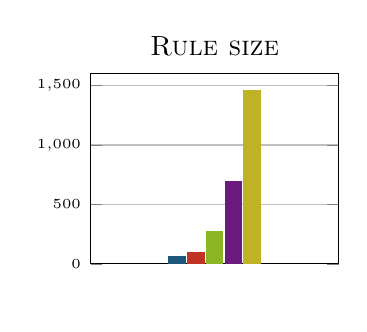
\begin{tikzpicture}
		    \begin{axis}[
		    black,
		        width  = 0.39*\textwidth,
		        height = \charth,
		        major x tick style = transparent,
		        ybar=2*\pgflinewidth,
		        bar width=6pt,
		        ymajorgrids = true,
		        ylabel = {\textsc{Rule size}},
		        every tick label/.append style={font=\tiny},
		        every axis x label/.style={
		        			white,
		  			  at={(ticklabel* cs:1.05)},
		  			  anchor=west,
		  			  },
					every axis y label/.style={at={(current axis.north)},above=1mm},
		        symbolic x coords={\textcolor{white}{abc}},
		        xtick = data,
		        scaled y ticks = false,
		        enlarge x limits=0,
		        ymin=0,
		        legend cell align=left,
		        legend style={
		        		at={(0.5,-0.15)},
						anchor=north,
						legend columns=-1
					},
		    ]
		    		\addplot[style={bblue,fill=bblue,mark=none}]
		            coordinates {(\textcolor{white}{abc}, 65)};
		        \addplot[style={rred,fill=rred,mark=none}]
		             coordinates {(\textcolor{white}{abc},95)};
		        \addplot[style={ggreen,fill=ggreen,mark=none}]
		             coordinates {(\textcolor{white}{abc},270)};
		        \addplot[style={ppurple,fill=ppurple,mark=none}]
		             coordinates {(\textcolor{white}{abc},690)};
		        \addplot[style={pyellow,fill=pyellow,mark=none}]
		             coordinates {(\textcolor{white}{abc},1456)};
		    \end{axis}
		\end{tikzpicture}
		\hspace*{1cm}
		% Computation Time
		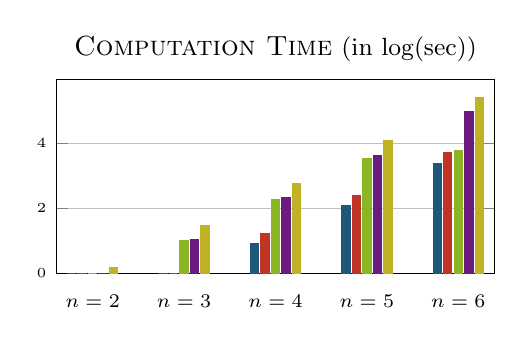
\begin{tikzpicture}
		    \begin{axis}[black,
		        width  = 0.59*\textwidth,
		        height = 1.01*\charth,
		        major x tick style = transparent,
		        ybar=2*\pgflinewidth,
		        bar width=3pt,
		        ymajorgrids = true,
		        ylabel = {\textsc{Computation Time} \small (in log(sec))},
		        %ytick={10^1, 2, 3, 4, 5, 6},
		        every tick label/.append style={font=\tiny},
		        every axis x label/.style={
		  			  at={(ticklabel* cs:1.05)},
		  			  anchor=west,
		  			  },
					every axis y label/.style={black, at={(current axis.north)},above=1mm},
		        symbolic x coords={\bb{2},\bb{3},\bb{4},\bb{5},\bb{6}},
		        xtick = data,
		        scaled y ticks = false,
		        enlarge x limits=0.1,
		        ymin=0,
		        legend cell align=left,
		        legend style={
		        		at={(0.5,-0.25)},
						anchor=north,
						legend columns=-1
					},
		    ]
				\addplot[style={bblue,fill=bblue,mark=none}]
		           coordinates {(\bb{2}, -1.5) (\bb{3},-0.3) (\bb{4},0.9) (\bb{5},2.1) (\bb{6},3.37)};

		        \addplot[style={rred,fill=rred,mark=none}]
		             coordinates {(\bb{2},-1.3) (\bb{3},0) (\bb{4},1.23) (\bb{5},2.39) (\bb{6},3.73)};

		        \addplot[style={ggreen,fill=ggreen,mark=none}]
		             coordinates {(\bb{2},-0.22) (\bb{3},1) (\bb{4},2.28) (\bb{5},3.54) (\bb{6},3.77)};

		        \addplot[style={ppurple,fill=ppurple,mark=none}]
		             coordinates {(\bb{2},-0.22) (\bb{3},1.04) (\bb{4},2.34) (\bb{5},3.64) (\bb{6},4.99)};

		        \addplot[style={pyellow,fill=pyellow,mark=none}]
		             coordinates {(\bb{2},0.17) (\bb{3},1.46) (\bb{4},2.77) (\bb{5},4.09) (\bb{6},5.42)};
		    \end{axis}
		\end{tikzpicture}
		\end{figure}
  	\end{frame}
    \metroset{background=dark}
    % -------------------------------------------------------------------------------------------------------
    
    \begin{frame}{Correspondences: Young Tableau}
    		\centering
		\setlength{\tabcolsep}{3\tabcolsep}
    		\begin{tabular}{lr}
    			\begin{tikzpicture}[every node/.style={anchor=base},xscale=.5]
				\node (n0) at (0,0) {$a_1$};
				\node (n1) at (1,0) {$a_2$};
				\node (n2) at (2,0) {$b_3$};
				\node (n3) at (3,0) {$b_4$};
				\node (n4) at (4,0) {$c_5$};
				\node (n5) at (5,0) {$c_6$};
				\draw (n0) edge [thick, mDarkTeal, bend left=90] (n2);
				\draw (n2) edge [thick, mDarkTeal, bend right=90] (n4);
			\end{tikzpicture} &
    			\begin{tikzpicture}[every node/.style={mDarkTeal}, every edge/.style={mDarkTeal},xscale=.5]
				\node (n0) at (0,0) {$a_1$};
				\node (n1) at (1,0) {$b_2$};
				\node (n2) at (2,0) {$a_3$};
				\node (n3) at (3,0) {$c_4$};
				\node (n4) at (4,0) {$b_5$};
				\node (n5) at (5,0) {$c_6$};
				\draw (n0) edge [thick, bend left=90] (n1);
				\draw (n1) edge [thick, bend right=90] (n3);
				\draw (n2) edge [thick, bend left=90] (n4);
				\draw (n4) edge [thick, bend right=90] (n5);
			\end{tikzpicture}\\
			\begin{tabular}{| c | c | c | c | c | c |}
		    		\hline
			    \rr{\textcolor{mDarkTeal}{1}} & \gr{\textcolor{mDarkTeal}{1}} \\
		    		\hline
			    \rr{\ } & \gr{\ } \\
			    \hline
			    \rr{\ } & \gr{\ } \\
		    		\hline
		    \end{tabular}
    		\end{tabular}
	\end{frame}
	
	\begin{frame}{Correspondences: Young Tableau}
		\centering
		\setlength{\tabcolsep}{3\tabcolsep}
    		\begin{tabular}{lr}
    			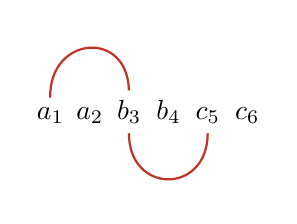
\begin{tikzpicture}[every node/.style={anchor=base},xscale=.5]
				\node (n0) at (0,0) {$a_1$};
				\node (n1) at (1,0) {$a_2$};
				\node (n2) at (2,0) {$b_3$};
				\node (n3) at (3,0) {$b_4$};
				\node (n4) at (4,0) {$c_5$};
				\node (n5) at (5,0) {$c_6$};
				\draw (n0) edge [thick, rred, bend left=90] (n2);
				\draw (n2) edge [thick, rred, bend right=90] (n4);
			\end{tikzpicture} &
    			\begin{tikzpicture}[every node/.style={mDarkTeal}, every edge/.style={mDarkTeal},xscale=.5]
				\node (n0) at (0,0) {$a_1$};
				\node (n1) at (1,0) {$b_2$};
				\node (n2) at (2,0) {$a_3$};
				\node (n3) at (3,0) {$c_4$};
				\node (n4) at (4,0) {$b_5$};
				\node (n5) at (5,0) {$c_6$};
				\draw (n0) edge [thick, bend left=90] (n1);
				\draw (n1) edge [thick, bend right=90] (n3);
				\draw (n2) edge [thick, bend left=90] (n4);
				\draw (n4) edge [thick, bend right=90] (n5);
			\end{tikzpicture}\\
			\begin{tabular}{| c | c | c | c | c | c |}
		    		\hline
			    \rr{1} & \textcolor{mDarkTeal}{1} \\
		    		\hline
			    \rr{3} & \ \\
			    \hline
			    \rr{5} & \ \\
		    		\hline
		    \end{tabular}
    		\end{tabular}
	\end{frame}
	\begin{frame}{Correspondences: Young Tableau}
		\centering
		\setlength{\tabcolsep}{3\tabcolsep}
    		\begin{tabular}{lr}
    			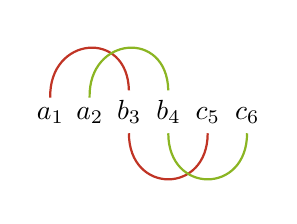
\begin{tikzpicture}[every node/.style={anchor=base},xscale=.5]
				\node (n0) at (0,0) {$a_1$};
				\node (n1) at (1,0) {$a_2$};
				\node (n2) at (2,0) {$b_3$};
				\node (n3) at (3,0) {$b_4$};
				\node (n4) at (4,0) {$c_5$};
				\node (n5) at (5,0) {$c_6$};
				\draw (n0) edge [thick, rred, bend left=90] (n2);
				\draw (n2) edge [thick, rred, bend right=90] (n4);
				\draw (n1) edge [thick, ggreen, bend left=90] (n3);
				\draw (n3) edge [thick, ggreen, bend right=90] (n5);
			\end{tikzpicture} &
    			\begin{tikzpicture}[every node/.style={mDarkTeal}, every edge/.style={mDarkTeal},xscale=.5]
				\node (n0) at (0,0) {$a_1$};
				\node (n1) at (1,0) {$b_2$};
				\node (n2) at (2,0) {$a_3$};
				\node (n3) at (3,0) {$c_4$};
				\node (n4) at (4,0) {$b_5$};
				\node (n5) at (5,0) {$c_6$};
				\draw (n0) edge [thick, bend left=90] (n1);
				\draw (n1) edge [thick, bend right=90] (n3);
				\draw (n2) edge [thick, bend left=90] (n4);
				\draw (n4) edge [thick, bend right=90] (n5);
			\end{tikzpicture}\\
			\begin{tabular}{| c | c | c | c | c | c |}
		    		\hline
			    \rr{1} & \gr{2} \\
		    		\hline
			    \rr{3} & \gr{4} \\
			    \hline
			    \rr{5} & \gr{6} \\
		    		\hline
		    \end{tabular}
    		\end{tabular}
	\end{frame}
	%-------------------------------------------- PRO
	\begin{frame}{Correspondences: Promotion on Young Tableaux}
		\centering
		\setlength{\tabcolsep}{3\tabcolsep}
    		\begin{tabular}{lr}
    			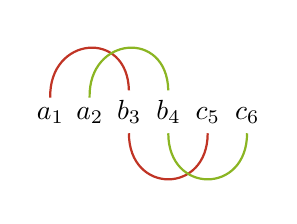
\begin{tikzpicture}[every node/.style={anchor=base},xscale=.5]
				\node (n0) at (0,0) {$a_1$};
				\node (n1) at (1,0) {$a_2$};
				\node (n2) at (2,0) {$b_3$};
				\node (n3) at (3,0) {$b_4$};
				\node (n4) at (4,0) {$c_5$};
				\node (n5) at (5,0) {$c_6$};
				\draw (n0) edge [thick, rred, bend left=90] (n2);
				\draw (n2) edge [thick, rred, bend right=90] (n4);
				\draw (n1) edge [thick, ggreen, bend left=90] (n3);
				\draw (n3) edge [thick, ggreen, bend right=90] (n5);
			\end{tikzpicture} &
    			\begin{tikzpicture}[every node/.style={mDarkTeal}, every edge/.style={mDarkTeal},xscale=.5]
				\node (n0) at (0,0) {$a_1$};
				\node (n1) at (1,0) {$b_2$};
				\node (n2) at (2,0) {$a_3$};
				\node (n3) at (3,0) {$c_4$};
				\node (n4) at (4,0) {$b_5$};
				\node (n5) at (5,0) {$c_6$};
				\draw (n0) edge [thick, bend left=90] (n1);
				\draw (n1) edge [thick, bend right=90] (n3);
				\draw (n2) edge [thick, bend left=90] (n4);
				\draw (n4) edge [thick, bend right=90] (n5);
			\end{tikzpicture}\\
			\begin{tabular}{| c | c | c | c | c | c |}
		    		\hline
			    \rr{1} & \gr{2} \\
		    		\hline
			    \rr{3} & \gr{4} \\
			    \hline
			    \rr{5} & \gr{6} \\
		    		\hline
		    \end{tabular} &
		    \begin{tabular}{| c | c | c | c | c | c |}
		    		\hline
			    \rr{\textcolor{mDarkTeal}{1}} & \gr{1} \\
		    		\hline
			    \rr{2} & \gr{3} \\
			    \hline
			    \rr{4} & \gr{5} \\
		    		\hline
		    \end{tabular}
    		\end{tabular}
	\end{frame}
	\begin{frame}{Correspondences: Promotion on Young Tableaux}
		\centering
		\setlength{\tabcolsep}{3\tabcolsep}
    		\begin{tabular}{lr}
    			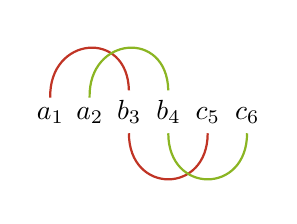
\begin{tikzpicture}[every node/.style={anchor=base},xscale=.5]
				\node (n0) at (0,0) {$a_1$};
				\node (n1) at (1,0) {$a_2$};
				\node (n2) at (2,0) {$b_3$};
				\node (n3) at (3,0) {$b_4$};
				\node (n4) at (4,0) {$c_5$};
				\node (n5) at (5,0) {$c_6$};
				\draw (n0) edge [thick, rred, bend left=90] (n2);
				\draw (n2) edge [thick, rred, bend right=90] (n4);
				\draw (n1) edge [thick, ggreen, bend left=90] (n3);
				\draw (n3) edge [thick, ggreen, bend right=90] (n5);
			\end{tikzpicture} &
    			\begin{tikzpicture}[every node/.style={mDarkTeal}, every edge/.style={mDarkTeal},xscale=.5]
				\node (n0) at (0,0) {$a_1$};
				\node (n1) at (1,0) {$b_2$};
				\node (n2) at (2,0) {$a_3$};
				\node (n3) at (3,0) {$c_4$};
				\node (n4) at (4,0) {$b_5$};
				\node (n5) at (5,0) {$c_6$};
				\draw (n0) edge [thick, bend left=90] (n1);
				\draw (n1) edge [thick, bend right=90] (n3);
				\draw (n2) edge [thick, bend left=90] (n4);
				\draw (n4) edge [thick, bend right=90] (n5);
			\end{tikzpicture}\\
			\begin{tabular}{| c | c | c | c | c | c |}
		    		\hline
			    \rr{1} & \gr{2} \\
		    		\hline
			    \rr{3} & \gr{4} \\
			    \hline
			    \rr{5} & \gr{6} \\
		    		\hline
		    \end{tabular} &
			\begin{tabular}{| c | c | c | c | c | c |}
		    		\hline
			    \rr{1} & \gr{\textcolor{mDarkTeal}{1}} \\
		    		\hline
			    \rr{2} & \gr{3} \\
			    \hline
			    \rr{4} & \gr{5} \\
		    		\hline
		    \end{tabular}
    		\end{tabular}
	\end{frame}
	\begin{frame}{Correspondences: Promotion on Young Tableaux}
		\centering
		\setlength{\tabcolsep}{3\tabcolsep}
    		\begin{tabular}{lr}
    			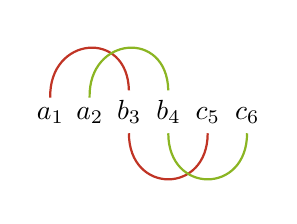
\begin{tikzpicture}[every node/.style={anchor=base},xscale=.5]
				\node (n0) at (0,0) {$a_1$};
				\node (n1) at (1,0) {$a_2$};
				\node (n2) at (2,0) {$b_3$};
				\node (n3) at (3,0) {$b_4$};
				\node (n4) at (4,0) {$c_5$};
				\node (n5) at (5,0) {$c_6$};
				\draw (n0) edge [thick, rred, bend left=90] (n2);
				\draw (n2) edge [thick, rred, bend right=90] (n4);
				\draw (n1) edge [thick, ggreen, bend left=90] (n3);
				\draw (n3) edge [thick, ggreen, bend right=90] (n5);
			\end{tikzpicture} &
    			\begin{tikzpicture}[every node/.style={mDarkTeal}, every edge/.style={mDarkTeal},xscale=.5]
				\node (n0) at (0,0) {$a_1$};
				\node (n1) at (1,0) {$b_2$};
				\node (n2) at (2,0) {$a_3$};
				\node (n3) at (3,0) {$c_4$};
				\node (n4) at (4,0) {$b_5$};
				\node (n5) at (5,0) {$c_6$};
				\draw (n0) edge [thick, bend left=90] (n1);
				\draw (n1) edge [thick, bend right=90] (n3);
				\draw (n2) edge [thick, bend left=90] (n4);
				\draw (n4) edge [thick, bend right=90] (n5);
			\end{tikzpicture}\\
			\begin{tabular}{| c | c | c | c | c | c |}
		    		\hline
			    \rr{1} & \gr{2} \\
		    		\hline
			    \rr{3} & \gr{4} \\
			    \hline
			    \rr{5} & \gr{6} \\
		    		\hline
		    \end{tabular} &
			\begin{tabular}{| c | c | c | c | c | c |}
		    		\hline
			    \rr{1} & \gr{3} \\
		    		\hline
			    \rr{2} & \gr{\textcolor{mDarkTeal}{1}} \\
			    \hline
			    \rr{4} & \gr{5} \\
		    		\hline
		    \end{tabular}
    		\end{tabular}
	\end{frame}	
	\begin{frame}{Correspondences: Promotion on Young Tableaux}
		\centering
		\setlength{\tabcolsep}{3\tabcolsep}
    		\begin{tabular}{lr}
    			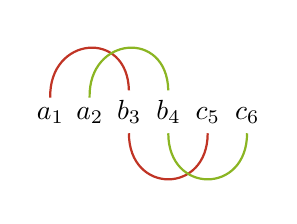
\begin{tikzpicture}[every node/.style={anchor=base},xscale=.5]
				\node (n0) at (0,0) {$a_1$};
				\node (n1) at (1,0) {$a_2$};
				\node (n2) at (2,0) {$b_3$};
				\node (n3) at (3,0) {$b_4$};
				\node (n4) at (4,0) {$c_5$};
				\node (n5) at (5,0) {$c_6$};
				\draw (n0) edge [thick, rred, bend left=90] (n2);
				\draw (n2) edge [thick, rred, bend right=90] (n4);
				\draw (n1) edge [thick, ggreen, bend left=90] (n3);
				\draw (n3) edge [thick, ggreen, bend right=90] (n5);
			\end{tikzpicture} &
    			\begin{tikzpicture}[every node/.style={mDarkTeal}, every edge/.style={mDarkTeal},xscale=.5]
				\node (n0) at (0,0) {$a_1$};
				\node (n1) at (1,0) {$b_2$};
				\node (n2) at (2,0) {$a_3$};
				\node (n3) at (3,0) {$c_4$};
				\node (n4) at (4,0) {$b_5$};
				\node (n5) at (5,0) {$c_6$};
				\draw (n0) edge [thick, bend left=90] (n1);
				\draw (n1) edge [thick, bend right=90] (n3);
				\draw (n2) edge [thick, bend left=90] (n4);
				\draw (n4) edge [thick, bend right=90] (n5);
			\end{tikzpicture}\\
			\begin{tabular}{| c | c | c | c | c | c |}
		    		\hline
			    \rr{1} & \gr{2} \\
		    		\hline
			    \rr{3} & \gr{4} \\
			    \hline
			    \rr{5} & \gr{6} \\
		    		\hline
		    \end{tabular} &
			\begin{tabular}{| c | c | c | c | c | c |}
		    		\hline
			    \rr{1} & \gr{3} \\
		    		\hline
			    \rr{2} & \gr{5} \\
			    \hline
			    \rr{4} & \gr{\textcolor{mDarkTeal}{1}} \\
		    		\hline
		    \end{tabular}
    		\end{tabular}
	\end{frame}		
	\begin{frame}{Correspondences: Promotion on Young Tableaux}
		\centering
		\setlength{\tabcolsep}{3\tabcolsep}
    		\begin{tabular}{lr}
    			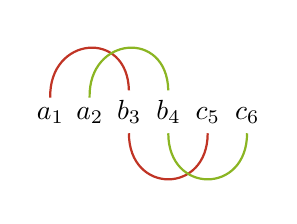
\begin{tikzpicture}[every node/.style={anchor=base},xscale=.5]
				\node (n0) at (0,0) {$a_1$};
				\node (n1) at (1,0) {$a_2$};
				\node (n2) at (2,0) {$b_3$};
				\node (n3) at (3,0) {$b_4$};
				\node (n4) at (4,0) {$c_5$};
				\node (n5) at (5,0) {$c_6$};
				\draw (n0) edge [thick, rred, bend left=90] (n2);
				\draw (n2) edge [thick, rred, bend right=90] (n4);
				\draw (n1) edge [thick, ggreen, bend left=90] (n3);
				\draw (n3) edge [thick, ggreen, bend right=90] (n5);
			\end{tikzpicture} &
    			\begin{tikzpicture}[every node/.style={mDarkTeal}, every edge/.style={mDarkTeal},xscale=.5]
				\node (n0) at (0,0) {$a_1$};
				\node (n1) at (1,0) {$b_2$};
				\node (n2) at (2,0) {$a_3$};
				\node (n3) at (3,0) {$c_4$};
				\node (n4) at (4,0) {$b_5$};
				\node (n5) at (5,0) {$c_6$};
				\draw (n0) edge [thick, bend left=90] (n1);
				\draw (n1) edge [thick, bend right=90] (n3);
				\draw (n2) edge [thick, bend left=90] (n4);
				\draw (n4) edge [thick, bend right=90] (n5);
			\end{tikzpicture}\\
			\begin{tabular}{| c | c | c | c | c | c |}
		    		\hline
			    \rr{1} & \gr{2} \\
		    		\hline
			    \rr{3} & \gr{4} \\
			    \hline
			    \rr{5} & \gr{6} \\
		    		\hline
		    \end{tabular} &
			\begin{tabular}{| c | c | c | c | c | c |}
		    		\hline
			    \rr{1} & \gr{3} \\
		    		\hline
			    \rr{2} & \gr{5} \\
			    \hline
			    \rr{4} & \gr{6} \\
		    		\hline
		    \end{tabular}
    		\end{tabular}
	\end{frame}
	\begin{frame}{Correspondences: Promotion on Young Tableaux}
		\centering
		\setlength{\tabcolsep}{3\tabcolsep}
    		\begin{tabular}{lr}
    			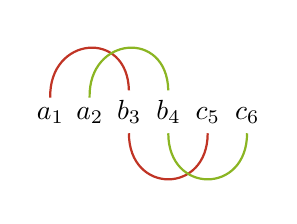
\begin{tikzpicture}[every node/.style={anchor=base},xscale=.5]
				\node (n0) at (0,0) {$a_1$};
				\node (n1) at (1,0) {$a_2$};
				\node (n2) at (2,0) {$b_3$};
				\node (n3) at (3,0) {$b_4$};
				\node (n4) at (4,0) {$c_5$};
				\node (n5) at (5,0) {$c_6$};
				\draw (n0) edge [thick, rred, bend left=90] (n2);
				\draw (n2) edge [thick, rred, bend right=90] (n4);
				\draw (n1) edge [thick, ggreen, bend left=90] (n3);
				\draw (n3) edge [thick, ggreen, bend right=90] (n5);
			\end{tikzpicture} &
    			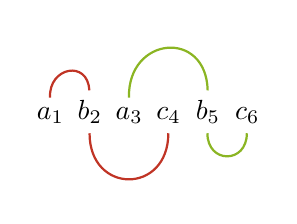
\begin{tikzpicture}[every node/.style={anchor=base},xscale=.5]
				\node (n0) at (0,0) {$a_1$};
				\node (n1) at (1,0) {$b_2$};
				\node (n2) at (2,0) {$a_3$};
				\node (n3) at (3,0) {$c_4$};
				\node (n4) at (4,0) {$b_5$};
				\node (n5) at (5,0) {$c_6$};
				\draw (n0) edge [thick, rred, bend left=90] (n1);
				\draw (n1) edge [thick, rred, bend right=90] (n3);
				\draw (n2) edge [thick, ggreen, bend left=90] (n4);
				\draw (n4) edge [thick, ggreen, bend right=90] (n5);
			\end{tikzpicture}\\
			\begin{tabular}{| c | c | c | c | c | c |}
		    		\hline
			    \rr{1} & \gr{2} \\
		    		\hline
			    \rr{3} & \gr{4} \\
			    \hline
			    \rr{5} & \gr{6} \\
		    		\hline
		    \end{tabular} &
			\begin{tabular}{| c | c | c | c | c | c |}
		    		\hline
			    \rr{1} & \gr{3} \\
		    		\hline
			    \rr{2} & \gr{5} \\
			    \hline
			    \rr{4} & \gr{6} \\
		    		\hline
		    \end{tabular}
    		\end{tabular}
	\end{frame}
	\begin{frame}{Correspondences: Spider Webs}
		\center \tsc{Growth rules}
		\vspace{-.6cm}
		\begin{figure}[h!]
			\[
			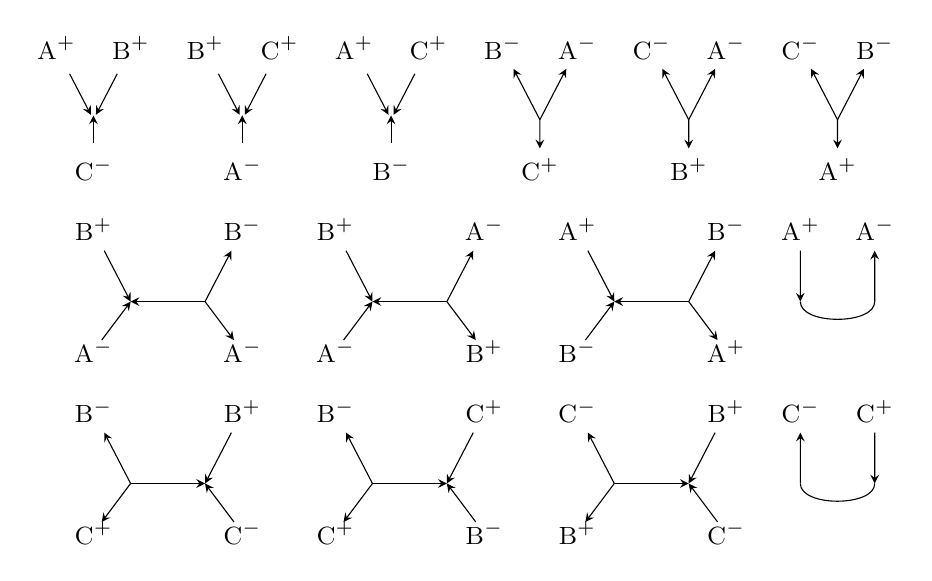
\begin{tikzpicture}[
			scale=.7,
			every node/.style={anchor=base},xscale=1.35,yscale=1.1,
			-->/.style={->,shorten >=2pt,shorten <=2pt,>=stealth},
			<--/.style={<-,shorten >=2pt,shorten <=2pt,>=stealth},
			--->/.style={->,shorten >=1pt,shorten <=1pt,>=stealth},
			<---/.style={<-,>=stealth},
			]
			\node (i1) at (0,0) {$\textsc{\small A}^+$};
			\node (ii1) at (1,0) {$\textsc{\small B}^+$};
			\node (d1) at (.5,-1) {};
			\node (o1) at (.5,-2) {$\textsc{\small C}^-$};
			\draw[-->] (i1) -- (d1.center);
			\draw[-->] (ii1) -- (d1.center);
			\draw[<--] (d1.north) -- (o1);
			
			\node (i2) at (2,0) {$\textsc{\small B}^+$};
			\node (ii2) at (3,0) {$\textsc{\small C}^+$};
			\node (d2) at (2.5,-1) {};
			\node (o2) at (2.5,-2) {$\textsc{\small A}^-$};
			\draw[-->] (i2) -- (d2.center);
			\draw[-->] (ii2) -- (d2.center);
			\draw[<--] (d2.north) -- (o2);
			
			\node (i3) at (4,0) {$\textsc{\small A}^+$};
			\node (ii3) at (5,0) {$\textsc{\small C}^+$};
			\node (d3) at (4.5,-1) {};
			\node (o3) at (4.5,-2) {$\textsc{\small B}^-$};
			\draw[-->] (i3) -- (d3.center);
			\draw[-->] (ii3) -- (d3.center);
			\draw[<--] (d3.north) -- (o3);
			
			\node (i4) at (6,0) {$\textsc{\small B}^-$};
			\node (ii4) at (7,0) {$\textsc{\small A}^-$};
			\node (d4) at (6.5,-1) {};
			\node (o4) at (6.5,-2) {$\textsc{\small C}^+$};
			\draw[<-,>=stealth] (i4) -- (d4.center);
			\draw[<-,>=stealth] (ii4) -- (d4.center);
			\draw[->,>=stealth] (d4.center) -- (o4);
			
			\node (i5) at (8,0) {$\textsc{\small C}^-$};
			\node (ii5) at (9,0) {$\textsc{\small A}^-$};
			\node (d5) at (8.5,-1) {};
			\node (o5) at (8.5,-2) {$\textsc{\small B}^+$};
			\draw[<-,>=stealth] (i5) -- (d5.center);
			\draw[<-,>=stealth] (ii5) -- (d5.center);
			\draw[->,>=stealth] (d5.center) -- (o5);
			
			\node (i6) at (10,0) {$\textsc{\small C}^-$};
			\node (ii6) at (11,0) {$\textsc{\small B}^-$};
			\node (d6) at (10.5,-1) {};
			\node (o6) at (10.5,-2) {$\textsc{\small A}^+$};
			\draw[<-,>=stealth] (i6) -- (d6.center);
			\draw[<-,>=stealth] (ii6) -- (d6.center);
			\draw[->,>=stealth] (d6.center) -- (o6);
			
			\node (i21) at (.5,-3) {$\textsc{\small B}^+$};
			\node (ii21) at (2.5,-3) {$\textsc{\small B}^-$};
			\node (d21) at (1,-4) {};
			\node (dd21) at (2,-4) {};
			\node (o21) at (.5,-5) {$\textsc{\small A}^-$};
			\node (oo21) at (2.5,-5) {$\textsc{\small A}^-$};
			\draw[->,>=stealth] (i21) -- (d21.center);
			\draw[<-,>=stealth] (ii21) -- (dd21.center);
			\draw[<-,>=stealth] (d21.center) -- (dd21.center);
			\draw[<-,>=stealth, shorten >=5pt] (d21.center) -- (o21.center);
			\draw[->,>=stealth, shorten >=5pt] (dd21.center) -- (oo21.center);
			
			\node (i22) at (3.75,-3) {$\textsc{\small B}^+$};
			\node (ii22) at (5.75,-3) {$\textsc{\small A}^-$};
			\node (d22) at (4.25,-4) {};
			\node (dd22) at (5.25,-4) {};
			\node (o22) at (3.75,-5) {$\textsc{\small A}^-$};
			\node (oo22) at (5.75,-5) {$\textsc{\small B}^+$};
			\draw[->,>=stealth] (i22) -- (d22.center);
			\draw[<-,>=stealth] (ii22) -- (dd22.center);
			\draw[<-,>=stealth] (d22.center) -- (dd22.center);
			\draw[<-,>=stealth, shorten >=5pt] (d22.center) -- (o22.center);
			\draw[->,>=stealth, shorten >=5pt] (dd22.center) -- (oo22.center);
			
			\node (i23) at (7,-3) {$\textsc{\small A}^+$};
			\node (ii23) at (9,-3) {$\textsc{\small B}^-$};
			\node (d23) at (7.5,-4) {};
			\node (dd23) at (8.5,-4) {};
			\node (o23) at (7,-5) {$\textsc{\small B}^-$};
			\node (oo23) at (9,-5) {$\textsc{\small A}^+$};
			\draw[->,>=stealth] (i23) -- (d23.center);
			\draw[<-,>=stealth] (ii23) -- (dd23.center);
			\draw[<-,>=stealth] (d23.center) -- (dd23.center);
			\draw[<-,>=stealth, shorten >=5pt] (d23.center) -- (o23.center);
			\draw[->,>=stealth, shorten >=5pt] (dd23.center) -- (oo23.center);
			
			\node (i24) at (10,-3) {$\textsc{\small A}^+$};
			\node (ii24) at (11,-3) {$\textsc{\small A}^-$};
			\node (d24) at (10,-4) {};
			\node (dd24) at (11,-4) {};
			\draw[->,>=stealth] (i24) -- (d24.center);
			\draw[<-,>=stealth] (ii24) -- (dd24.center);
			\draw (d24.center) edge [-,>=stealth,bend right=90] (dd24.center);
			
			\node (i31) at (.5,-6) {$\textsc{\small B}^-$};
			\node (ii31) at (2.5,-6) {$\textsc{\small B}^+$};
			\node (d31) at (1,-7) {};
			\node (dd31) at (2,-7) {};
			\node (o31) at (.5,-8) {$\textsc{\small C}^+$};
			\node (oo31) at (2.5,-8) {$\textsc{\small C}^-$};
			\draw[<-,>=stealth] (i31) -- (d31.center);
			\draw[->,>=stealth] (ii31) -- (dd31.center);
			\draw[->,>=stealth] (d31.center) -- (dd31.center);
			\draw[->,>=stealth, shorten >=5pt] (d31.center) -- (o31.center);
			\draw[<-,>=stealth, shorten >=5pt] (dd31.center) -- (oo31.center);
			
			\node (i32) at (3.75,-6) {$\textsc{\small B}^-$};
			\node (ii32) at (5.75,-6) {$\textsc{\small C}^+$};
			\node (d32) at (4.25,-7) {};
			\node (dd32) at (5.25,-7) {};
			\node (o32) at (3.75,-8) {$\textsc{\small C}^+$};
			\node (oo32) at (5.75,-8) {$\textsc{\small B}^-$};
			\draw[<-,>=stealth] (i32) -- (d32.center);
			\draw[->,>=stealth] (ii32) -- (dd32.center);
			\draw[->,>=stealth] (d32.center) -- (dd32.center);
			\draw[->,>=stealth, shorten >=5pt] (d32.center) -- (o32.center);
			\draw[<-,>=stealth, shorten >=5pt] (dd32.center) -- (oo32.center);
			
			\node (i33) at (7,-6) {$\textsc{\small C}^-$};
			\node (ii33) at (9,-6) {$\textsc{\small B}^+$};
			\node (d33) at (7.5,-7) {};
			\node (dd33) at (8.5,-7) {};
			\node (o33) at (7,-8) {$\textsc{\small B}^+$};
			\node (oo33) at (9,-8) {$\textsc{\small C}^-$};
			\draw[<-,>=stealth] (i33) -- (d33.center);
			\draw[->,>=stealth] (ii33) -- (dd33.center);
			\draw[->,>=stealth] (d33.center) -- (dd33.center);
			\draw[->,>=stealth, shorten >=5pt] (d33.center) -- (o33.center);
			\draw[<-,>=stealth, shorten >=5pt] (dd33.center) -- (oo33.center);
			
			\node (i34) at (10,-6) {$\textsc{\small C}^-$};
			\node (ii34) at (11,-6) {$\textsc{\small C}^+$};
			\node (d34) at (10,-7) {};
			\node (dd34) at (11,-7) {};
			\draw[<-,>=stealth] (i34) -- (d34.center);
			\draw[->,>=stealth] (ii34) -- (dd34.center);
			\draw (d34.center) edge [-,>=stealth,bend right=90] (dd34.center);
			
			\end{tikzpicture}
			\]
			\end{figure}
	\end{frame}
	\begin{frame}{}
		\epigraph
			{When you depart for Ithaca,\\wish for the road to be long,\\full of adventure, full of knowledge.}
			{\textit{C. P. Cavafy\\ Ithaca}}
	\end{frame}
  	
\end{document}
